
%% bare_conf.tex
%% V1.4
%% 2012/12/27
%% by Michael Shell
%% See:
%% http://www.michaelshell.org/
%% for current contact information.
%%
%% This is a skeleton file demonstrating the use of IEEEtran.cls
%% (requires IEEEtran.cls version 1.8 or later) with an IEEE conference paper.
%%
%% Support sites:
%% http://www.michaelshell.org/tex/ieeetran/
%% http://www.ctan.org/tex-archive/macros/latex/contrib/IEEEtran/
%% and
%% http://www.ieee.org/

%%*************************************************************************
%% Legal Notice:
%% This code is offered as-is without any warranty either expressed or
%% implied; without even the implied warranty of MERCHANTABILITY or
%% FITNESS FOR A PARTICULAR PURPOSE! 
%% User assumes all risk.
%% In no event shall IEEE or any contributor to this code be liable for
%% any damages or losses, including, but not limited to, incidental,
%% consequential, or any other damages, resulting from the use or misuse
%% of any information contained here.
%%
%% All comments are the opinions of their respective authors and are not
%% necessarily endorsed by the IEEE.
%%
%% This work is distributed under the LaTeX Project Public License (LPPL)
%% ( http://www.latex-project.org/ ) version 1.3, and may be freely used,
%% distributed and modified. A copy of the LPPL, version 1.3, is included
%% in the base LaTeX documentation of all distributions of LaTeX released
%% 2003/12/01 or later.
%% Retain all contribution notices and credits.
%% ** Modified files should be clearly indicated as such, including  **
%% ** renaming them and changing author support contact information. **
%%
%% File list of work: IEEEtran.cls, IEEEtran_HOWTO.pdf, bare_adv.tex,
%%                    bare_conf.tex, bare_jrnl.tex, bare_jrnl_compsoc.tex,
%%                    bare_jrnl_transmag.tex
%%*************************************************************************

% *** Authors should verify (and, if needed, correct) their LaTeX system  ***
% *** with the testflow diagnostic prior to trusting their LaTeX platform ***
% *** with production work. IEEE's font choices can trigger bugs that do  ***
% *** not appear when using other class files.                            ***
% The testflow support page is at:
% http://www.michaelshell.org/tex/testflow/



% Note that the a4paper option is mainly intended so that authors in
% countries using A4 can easily print to A4 and see how their papers will
% look in print - the typesetting of the document will not typically be
% affected with changes in paper size (but the bottom and side margins will).
% Use the testflow package mentioned above to verify correct handling of
% both paper sizes by the user's LaTeX system.
%
% Also note that the "draftcls" or "draftclsnofoot", not "draft", option
% should be used if it is desired that the figures are to be displayed in
% draft mode.
%
\documentclass[12pt,a4paper,final]{article}
%\documentclass[conference]{IEEEtrans}
% Add the compsoc option for Computer Society conferences.
%
% If IEEEtran.cls has not been installed into the LaTeX system files,
% manually specify the path to it like:
\usepackage[latin1]{inputenc}
\usepackage{amsfonts}
\usepackage{amssymb}
\usepackage{amsthm}
\usepackage{fullpage}
\usepackage{setspace}
\usepackage{graphicx}
%\usepackage[pdftex]{graphicx}
\usepackage{psfrag}
\usepackage{color}
\usepackage{epsfig}
\usepackage{appendix}
\usepackage{caption}
\usepackage{cite}
\usepackage{ifpdf}
\usepackage[cmex10]{amsmath}
\usepackage{algorithmic}
\usepackage{array}
\usepackage{stfloats}
\usepackage{url}
\usepackage{fixltx2e}
\usepackage{setspace} 
\usepackage{multirow}




% Some very useful LaTeX packages include:
% (uncomment the ones you want to load)


% *** MISC UTILITY PACKAGES ***
%
%\usepackage{ifpdf}
% Heiko Oberdiek's ifpdf.sty is very useful if you need conditional
% compilation based on whether the output is pdf or dvi.
% usage:
% \ifpdf
%   % pdf code
% \else
%   % dvi code
% \fi
% The latest version of ifpdf.sty can be obtained from:
% http://www.ctan.org/tex-archive/macros/latex/contrib/oberdiek/
% Also, note that IEEEtran.cls V1.7 and later provides a builtin
% \ifCLASSINFOpdf conditional that works the same way.
% When switching from latex to pdflatex and vice-versa, the compiler may
% have to be run twice to clear warning/error messages.






% *** CITATION PACKAGES ***
%
%\usepackage{cite}
% cite.sty was written by Donald Arseneau
% V1.6 and later of IEEEtran pre-defines the format of the cite.sty package
% \cite{} output to follow that of IEEE. Loading the cite package will
% result in citation numbers being automatically sorted and properly
% "compressed/ranged". e.g., [1], [9], [2], [7], [5], [6] without using
% cite.sty will become [1], [2], [5]--[7], [9] using cite.sty. cite.sty's
% \cite will automatically add leading space, if needed. Use cite.sty's
% noadjust option (cite.sty V3.8 and later) if you want to turn this off
% such as if a citation ever needs to be enclosed in parenthesis.
% cite.sty is already installed on most LaTeX systems. Be sure and use
% version 4.0 (2003-05-27) and later if using hyperref.sty. cite.sty does
% not currently provide for hyperlinked citations.
% The latest version can be obtained at:
% http://www.ctan.org/tex-archive/macros/latex/contrib/cite/
% The documentation is contained in the cite.sty file itself.






% *** GRAPHICS RELATED PACKAGES ***
%
%\ifCLASSINFOpdf
  % \usepackage[pdftex]{graphicx}
  % declare the path(s) where your graphic files are
  % \graphicspath{{../pdf/}{../jpeg/}}
  % and their extensions so you won't have to specify these with
  % every instance of \includegraphics
  % \DeclareGraphicsExtensions{.pdf,.jpeg,.png}
%\else
  % or other class option (dvipsone, dvipdf, if not using dvips). graphicx
  % will default to the driver specified in the system graphics.cfg if no
  % driver is specified.
  % \usepackage[dvips]{graphicx}
  % declare the path(s) where your graphic files are
  % \graphicspath{{../eps/}}
  % and their extensions so you won't have to specify these with
  % every instance of \includegraphics
  % \DeclareGraphicsExtensions{.eps}
%\fi
% graphicx was written by David Carlisle and Sebastian Rahtz. It is
% required if you want graphics, photos, etc. graphicx.sty is already
% installed on most LaTeX systems. The latest version and documentation
% can be obtained at: 
% http://www.ctan.org/tex-archive/macros/latex/required/graphics/
% Another good source of documentation is "Using Imported Graphics in
% LaTeX2e" by Keith Reckdahl which can be found at:
% http://www.ctan.org/tex-archive/info/epslatex/
%
% latex, and pdflatex in dvi mode, support graphics in encapsulated
% postscript (.eps) format. pdflatex in pdf mode supports graphics
% in .pdf, .jpeg, .png and .mps (metapost) formats. Users should ensure
% that all non-photo figures use a vector format (.eps, .pdf, .mps) and
% not a bitmapped formats (.jpeg, .png). IEEE frowns on bitmapped formats
% which can result in "jaggedy"/blurry rendering of lines and letters as
% well as large increases in file sizes.
%
% You can find documentation about the pdfTeX application at:
% http://www.tug.org/applications/pdftex





% *** MATH PACKAGES ***
%
%\usepackage[cmex10]{amsmath}
% A popular package from the American Mathematical Society that provides
% many useful and powerful commands for dealing with mathematics. If using
% it, be sure to load this package with the cmex10 option to ensure that
% only type 1 fonts will utilized at all point sizes. Without this option,
% it is possible that some math symbols, particularly those within
% footnotes, will be rendered in bitmap form which will result in a
% document that can not be IEEE Xplore compliant!
%
% Also, note that the amsmath package sets \interdisplaylinepenalty to 10000
% thus preventing page breaks from occurring within multiline equations. Use:
%\interdisplaylinepenalty=2500
% after loading amsmath to restore such page breaks as IEEEtran.cls normally
% does. amsmath.sty is already installed on most LaTeX systems. The latest
% version and documentation can be obtained at:
% http://www.ctan.org/tex-archive/macros/latex/required/amslatex/math/





% *** SPECIALIZED LIST PACKAGES ***
%
%\usepackage{algorithmic}
% algorithmic.sty was written by Peter Williams and Rogerio Brito.
% This package provides an algorithmic environment fo describing algorithms.
% You can use the algorithmic environment in-text or within a figure
% environment to provide for a floating algorithm. Do NOT use the algorithm
% floating environment provided by algorithm.sty (by the same authors) or
% algorithm2e.sty (by Christophe Fiorio) as IEEE does not use dedicated
% algorithm float types and packages that provide these will not provide
% correct IEEE style captions. The latest version and documentation of
% algorithmic.sty can be obtained at:
% http://www.ctan.org/tex-archive/macros/latex/contrib/algorithms/
% There is also a support site at:
% http://algorithms.berlios.de/index.html
% Also of interest may be the (relatively newer and more customizable)
% algorithmicx.sty package by Szasz Janos:
% http://www.ctan.org/tex-archive/macros/latex/contrib/algorithmicx/




% *** ALIGNMENT PACKAGES ***
%
%\usepackage{array}
% Frank Mittelbach's and David Carlisle's array.sty patches and improves
% the standard LaTeX2e array and tabular environments to provide better
% appearance and additional user controls. As the default LaTeX2e table
% generation code is lacking to the point of almost being broken with
% respect to the quality of the end results, all users are strongly
% advised to use an enhanced (at the very least that provided by array.sty)
% set of table tools. array.sty is already installed on most systems. The
% latest version and documentation can be obtained at:
% http://www.ctan.org/tex-archive/macros/latex/required/tools/


% IEEEtran contains the IEEEeqnarray family of commands that can be used to
% generate multiline equations as well as matrices, tables, etc., of high
% quality.




% *** SUBFIGURE PACKAGES ***
%\ifCLASSOPTIONcompsoc
%  \usepackage[caption=false,font=normalsize,labelfont=sf,textfont=sf]{subfig}
%\else
%  \usepackage[caption=false,font=footnotesize]{subfig}
%\fi
% subfig.sty, written by Steven Douglas Cochran, is the modern replacement
% for subfigure.sty, the latter of which is no longer maintained and is
% incompatible with some LaTeX packages including fixltx2e. However,
% subfig.sty requires and automatically loads Axel Sommerfeldt's caption.sty
% which will override IEEEtran.cls' handling of captions and this will result
% in non-IEEE style figure/table captions. To prevent this problem, be sure
% and invoke subfig.sty's "caption=false" package option (available since
% subfig.sty version 1.3, 2005/06/28) as this is will preserve IEEEtran.cls
% handling of captions.
% Note that the Computer Society format requires a larger sans serif font
% than the serif footnote size font used in traditional IEEE formatting
% and thus the need to invoke different subfig.sty package options depending
% on whether compsoc mode has been enabled.
%
% The latest version and documentation of subfig.sty can be obtained at:
% http://www.ctan.org/tex-archive/macros/latex/contrib/subfig/




% *** FLOAT PACKAGES ***
%
%\usepackage{fixltx2e}
% fixltx2e, the successor to the earlier fix2col.sty, was written by
% Frank Mittelbach and David Carlisle. This package corrects a few problems
% in the LaTeX2e kernel, the most notable of which is that in current
% LaTeX2e releases, the ordering of single and double column floats is not
% guaranteed to be preserved. Thus, an unpatched LaTeX2e can allow a
% single column figure to be placed prior to an earlier double column
% figure. The latest version and documentation can be found at:
% http://www.ctan.org/tex-archive/macros/latex/base/


%\usepackage{stfloats}
% stfloats.sty was written by Sigitas Tolusis. This package gives LaTeX2e
% the ability to do double column floats at the bottom of the page as well
% as the top. (e.g., "\begin{figure*}[!b]" is not normally possible in
% LaTeX2e). It also provides a command:
%\fnbelowfloat
% to enable the placement of footnotes below bottom floats (the standard
% LaTeX2e kernel puts them above bottom floats). This is an invasive package
% which rewrites many portions of the LaTeX2e float routines. It may not work
% with other packages that modify the LaTeX2e float routines. The latest
% version and documentation can be obtained at:
% http://www.ctan.org/tex-archive/macros/latex/contrib/sttools/
% Do not use the stfloats baselinefloat ability as IEEE does not allow
% \baselineskip to stretch. Authors submitting work to the IEEE should note
% that IEEE rarely uses double column equations and that authors should try
% to avoid such use. Do not be tempted to use the cuted.sty or midfloat.sty
% packages (also by Sigitas Tolusis) as IEEE does not format its papers in
% such ways.
% Do not attempt to use stfloats with fixltx2e as they are incompatible.
% Instead, use Morten Hogholm'a dblfloatfix which combines the features
% of both fixltx2e and stfloats:
%
% \usepackage{dblfloatfix}
% The latest version can be found at:
% http://www.ctan.org/tex-archive/macros/latex/contrib/dblfloatfix/




% *** PDF, URL AND HYPERLINK PACKAGES ***
%
%\usepackage{url}
% url.sty was written by Donald Arseneau. It provides better support for
% handling and breaking URLs. url.sty is already installed on most LaTeX
% systems. The latest version and documentation can be obtained at:
% http://www.ctan.org/tex-archive/macros/latex/contrib/url/
% Basically, \url{my_url_here}.




% *** Do not adjust lengths that control margins, column widths, etc. ***
% *** Do not use packages that alter fonts (such as pslatex).         ***
% There should be no need to do such things with IEEEtran.cls V1.6 and later.
% (Unless specifically asked to do so by the journal or conference you plan
% to submit to, of course. )


% correct bad hyphenation here
%\hyphenation{op-tical net-works semi-conduc-tor}



%
% paper title
% can use linebreaks \\ within to get better formatting as desired
% Do not put math or special symbols in the title.
\title{Parallel Acceleration of Fixed Complexity Sphere Decoder for Large MIMO Uplink System based on GPU}


% author names and affiliations
% use a multiple column layout for up to three different
% affiliations
%\author{\IEEEauthorblockN{Tianpei Chen}
%\IEEEauthorblockA{ID: 25504946\\Department of Electrical and\\Computer Engineering\\
%McGill University\\
%Montreal, Quebec}}
\author{Tianpei Chen, Harry Leib\\
 Department of Electrical and Computer Engineering\\
 McGill University\\
 Montreal, Quebec}

% conference papers do not typically use \thanks and this command
% is locked out in conference mode. If really needed, such as for
% the acknowledgment of grants, issue a \IEEEoverridecommandlockouts
% after \documentclass

% for over three affiliations, or if they all won't fit within the width
% of the page, use this alternative format:
% 
%\author{\IEEEauthorblockN{Michael Shell\IEEEauthorrefmark{1},
%Homer Simpson\IEEEauthorrefmark{2},
%James Kirk\IEEEauthorrefmark{3}, 
%Montgomery Scott\IEEEauthorrefmark{3} and
%Eldon Tyrell\IEEEauthorrefmark{4}}
%\IEEEauthorblockA{\IEEEauthorrefmark{1}School of Electrical and Computer Engineering\\
%Georgia Institute of Technology,
%Atlanta, Georgia 30332--0250\\ Email: see http://www.michaelshell.org/contact.html}
%\IEEEauthorblockA{\IEEEauthorrefmark{2}Twentieth Century Fox, Springfield, USA\\
%Email: homer@thesimpsons.com}
%\IEEEauthorblockA{\IEEEauthorrefmark{3}Starfleet Academy, San Francisco, California 96678-2391\\
%Telephone: (800) 555--1212, Fax: (888) 555--1212}
%\IEEEauthorblockA{\IEEEauthorrefmark{4}Tyrell Inc., 123 Replicant Street, Los Angeles, California 90210--4321}}




% use for special paper notices
%\IEEEspecialpapernotice{(Invited Paper)}



\begin{document}
% make the title area
\begin{spacing}{2.5}
\maketitle

% As a general rule, do not put math, special symbols or citations
% in the abstract
\begin{abstract}
The large MIMO system which is a scaling up of conventional MIMO systems with several hundreds of antennas at the base station serving several tens of terminals at the same time,  which is thought to be a big idea for the next generation wireless communication system. However the detection of the large MIMO system acquires a long time to get optimum or sub-optimum solutions, In order to accelerate the real-time decoder for large MIMO system, in this paper we present General Purpose Graphic Processing Units (GPGPU) implementation of Fixed Complexity Sphere Decoder (FCSD) for the large scale MIMO system based on the dominant propriety framework of GPGPU-Computed Unified Device Architecture (CUDA). The simulation shows a up to nearly $5$ times acceleration for $32\times 32$ array of whole application CPU version, furthermore, the proposed CUDA-FCSD algorithm shows a increasing speedup performance for a increasing array size. 
\end{abstract}

% no keywords




% For peer review papers, you can put extra information on the cover
% page as needed:
% \ifCLASSOPTIONpeerreview
% \begin{center} \bfseries EDICS Category: 3-BBND \end{center}
% \fi
%
% For peerreview papers, this IEEEtran command inserts a page break and
% creates the second title. It will be ignored for other modes.
%\IEEEpeerreviewmaketitle

\section{Introduction}
 The common challenge that all the researchers, engineers and industrial companies are now facing in wireless communication area is the sharp contrast between the increasing demand of the mobile network speed for the transmission of rich media content and better QoS (quality of service) and the limited bandwidth of the radio frequency spectrum and a complex space time varying wireless environment, moreover in foreseeable future this demand will continue grow. Multiple Input Multiple Output (MIMO) has become a very promising technology that can help to solve this problem, the core idea of MIMO is to use multiple antennas both at the transmitting end and receiving end, the spatial domain sampled signal can be combined to provide parallel data pipes so that it can provide array gain, spatial diversity gain, spatial multiplexing gain, and interference reduction\cite{oestges2010mimo}. LTE standard support up to 8 antennas at the base station\cite{dahlman20103g}, The large scale MIMO (also named massive MIMO) is a system with hundreds of low-power low-price antennas collocated at the base station and serving several tens of terminals at the same time\cite{rusek2013scaling}, originated from multiuser MIMO (MU-MIMO)\cite{larsson2013massive}. Large scale MIMO will inherit and enhance all the advantages of conventional MIMO (array gain, spatial diversity gain, spatial multiplexing gain and interference reduction), as well as reduction of latency, improvement of the whole system robustness. 
 As a classical list based decoder for MIMO system, Sphere decoder (SD) can reach the optimum diversity gain as maximum likelihood (ML) detection with a dramatic complexity reduction\cite{viterbo1999universal}\cite{hassibi2005sphere}, however, there are two major problems of this decoder is the varied complexity with signal to noise ratio and sequential nature, which is contradictory with the requirement of a constant data processing throughput and parallel implementation for practical system. Fixed Complexity Sphere Decoder (FCSD), overcomes this two disadvantage of the SD by searching the solution along the fixed number independent multiple paths\cite{barbero2008fixing}.
GPGPU (General purpose Graphic processing Units Computing) has become a big idea in the industry and research of a variety of areas that needs massive data analysis and computation such as computer vision\cite{fung2008using}, computer games\cite{blewitt2013applicability}, signal processing\cite{van2011accelerating}\cite{6671435} and finance\cite{grauer2013accelerating}. Comparing to CPU, The GPU has been designed as computational intensive, with most of the hardware resource be allocated for data processing and parallel computation rather than caching and flow control. In recent years GPU has reached huge advantages in data processing speed over CPU\cite{nvidia2008programming}.  CUDA (Computed unified Device Architecture) is a programming model for GPGPU that proposed by Nvidia which has becoming the dominant proprietary framework for GPGPU programming, it is based on popular programming languages(C, C++, java, python, Fortran, Direct Compute) so that the application developers in different areas do not need to learn a new programming language or get to know the hardware details. The core essence of the CUDA is the Single Instruction Multiple Threads (SIMT) programming model, enables GPU can accelerate a lot of applications with the large dataset by implementing parallel data processing of complex computations. CUDA has become a parallel computing platform for wide community of different application developers in different areas.  
\section{MIMO System Model}\label{system}
% no \IEEEPARstart
%This demo file is intended to serve as a ``starter file''
%for IEEE conference papers produced under \LaTeX\ using
%IEEEtran.cls version 1.8 and later.
% You must have at least 2 lines in the paragraph with the drop letter
% (should never be an issue)
%I wish you the best of success.
%\hfill mds
%\hfill December 27, 2012
We consider a complex uncoded spatial multiplexing MIMO system with $N_r$ receive antennas and $N_t$ transmit antennas, $N_{r}\geq N_{t}$, in the flat fading channel the corresponding discrete time model is given:
\begin{equation}
y=\mathbf{H}s+n   \label{formula 1}
\end{equation}
$s\in \mathbb{C}^{N_{t}\times 1}$ is the transmit symbol vector, the symbol in $s$ are mutually independent and taken from the signal constellation $\mathbb{O}$ (BPSK, QPSK, M-QAM), $M$ is the signal constellation size, all the transmit symbol vectors forms a $N_{t}$-dimensional signal constellation $\mathbb{O}^{N_{t}}$. $\varepsilon[ss^{H}]=I_{N_t}E_{s}$, $E_{s}$ denotes the symbol average energy where $\varepsilon$ denotes the mean operation.  $y\in \mathbb{C}^{N_{r}\times 1}$ is the receive symbol vector, $\mathbf{H}\in \mathbb{C}^{N_{r}\times N_{t}}$ denotes the Rayleigh fading channel propagation matrix with independent identity distributed(i.i.d) circularly symmetric complex Gaussian zero mean elements of unit variance, $n\in \mathbb{C}^{N_{r}\times 1}$ is the additive white Gaussian noise (AWGN) samples with zero mean elements of variance $\varepsilon[nn^{H}]=I_{N_{r}}N_{0}$, $N_{0}$ denotes the average noise energy, $\frac{E_{s}}{N_{0}}$ denotes the signal to noise ratio (SNR). \\
  Assume we have the perfect channel state information (CSI)  $\quad \mathbf{H}$, receive symbol vector $y$, and we had already known the SNR, the task of decoder for MIMO system is to estimate $s$ in \ref{formula 1} based on CSI and received signal.

% An example of a floating figure using the graphicx package.
% Note that \label must occur AFTER (or within) \caption.

% For figures, \caption should occur after the \includegraphics.
% Note that IEEEtran v1.7 and later has special internal code that
% is designed to preserve the operation of \label within \caption
% even when the captionsoff option is in effect. However, because
% of issues like this, it may be the safest practice to put all your
% \label just after \caption rather than within \caption{}.
%
% Reminder: the "draftcls" or "draftclsnofoot", not "draft", class
% option should be used if it is desired that the figures are to be
% displayed while in draft mode.
%
%\begin{figure}[!t]
%\centering
%\includegraphics[width=2.5in]{myfigure}
% where an .eps filename suffix will be assumed under latex, 
% and a .pdf suffix will be assumed for pdflatex; or what has been declared
% via \DeclareGraphicsExtensions.
%\caption{Simulation Results.}
%\label{fig_sim}
%\end{figure}

% Note that IEEE typically puts floats only at the top, even when this
% results in a large percentage of a column being occupied by floats.


% An example of a double column floating figure using two subfigures.
% (The subfig.sty package must be loaded for this to work.)
% The subfigure \label commands are set within each subfloat command,
% and the \label for the overall figure must come after \caption.
% \hfil is used as a separator to get equal spacing.
% Watch out that the combined width of all the subfigures on a 
% line do not exceed the text width or a line break will occur.
%
%\begin{figure*}[!t]
%\centering
%\subfloat[Case I]{\includegraphics[width=2.5in]{box}%
%\label{fig_first_case}}
%\hfil
%\subfloat[Case II]{\includegraphics[width=2.5in]{box}%
%\label{fig_second_case}}
%\caption{Simulation results.}
%\label{fig_sim}
%\end{figure*}
%
% Note that often IEEE papers with subfigures do not employ subfigure
% captions (using the optional argument to \subfloat[]), but instead will
% reference/describe all of them (a), (b), etc., within the main caption.


% An example of a floating table. Note that, for IEEE style tables, the 
% \caption command should come BEFORE the table. Table text will default to
% \footnotesize as IEEE normally uses this smaller font for tables.
% The \label must come after \caption as always.
%
%\begin{table}[!t]
%% increase table row spacing, adjust to taste
%\renewcommand{\arraystretch}{1.3}
% if using array.sty, it might be a good idea to tweak the value of
% \extrarowheight as needed to properly center the text within the cells
%\caption{An Example of a Table}
%\label{table_example}
%\centering
%% Some packages, such as MDW tools, offer better commands for making tables
%% than the plain LaTeX2e tabular which is used here.
%\begin{tabular}{|c||c|}
%\hline
%One & Two\\
%\hline
%Three & Four\\
%\hline
%\end{tabular}
%\end{table}

\section{CUDA GPU Architecture and  Programming Model} \label{programming model}
  CUDA programming model is the C programming extension, with special defined syntax and structure, CUDA divide the CPU and GPU as host and device, the serial code executes on the host (CPU) side and parallel data processing is performed on the device (GPU) side, which is defined as heterogeneous programming model. The code executes on the device side is defined as $\mathit{kernel}$ function, which is a single instruction invoked at host side but with a massive parallel data processing threads execution on the device (SIMT), This programming architecture is askin to Single Instruction Multiple Data (SIMD), however unlike the SIMD vectoring machines, SIMT can branching the behavior of each threads so that reach thread-level parallelism, thread is the basic programming unit of CUDA, a block of cooperative threads form a thread block, in one block all the threads can share a memory called shared memory that all the threads in the block have the access to this pitch of memory, the GPU use massive number of threads to hide the long latency of global memory instead of using large cache as CPU, Another function of the thread block is all the thread execute in one block can synchronize their action. The warp is the basic schedule unit with a constant number of threads  (for current version of CUDA device, the warp size is 32), when one warp are waiting for data loading the other warps just begin to execute. In a word CPU cores are designed to minimize latency for each thread at a time , whereas GPUs are designed to handle a large number of concurrent, lightweight threads in order to maximize throughput. Blocks are grouped into a one-dimensional, two-dimensional, or three-dimensional grid, similarly, one thread block can also be organized into one-dimentional, two-dimensional or three-dimensional. The organization of the block and grid shape and dimension is determined by the concrete application, Figure \ref{figure1} shows the 3 dimensional thread hierarchy of CUDA.
\begin{figure}[htb]
\centering
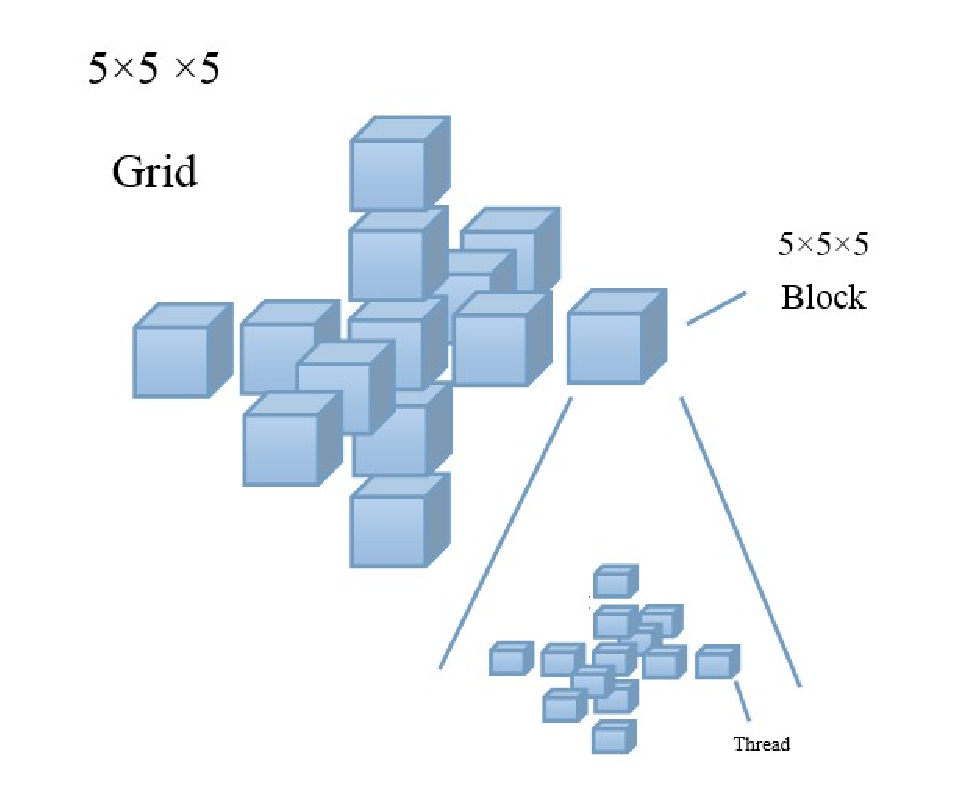
\includegraphics[scale=0.5]{CUDA_programming_hierachy.eps}
\caption{CUDA 3D thread hierachy\\ $5\times 5\times 5$ grid and each block contains $5\times 5\times 5$ threads\\}
\label{figure1}
\end{figure}
In Figure \ref{figure2} we use the GPU-GeForce GTX 760 as an example to show the microarchitecture of  GPU. The GPU works as a coprocessor system, consists of Stream Multiprocessors (SM), GeForce GTX 760 has 6 SM performs the multiply-add arithmetic operation and furthermore, each SM has the special functional units(SFU) that can perform more complex arithmetic operation such as trigonometric functions and reciprocal square root. the shared memory is also called on-chip memory which is located at SM that has low latency and limited capacity. Global memory, which is off-chip located memory of GPU with long latency and large capacity, another two types of the memory is called texture memory and constant memory, which are located off-chip , but cached, therefore the loading speed of the data located at these two type of memory space will be much faster than the that from global memory, for constant memory, it is read only and the memory latency is approximately as small as the registers.  The variables invoked in kernel functions can be stored in either of the these 4 types of memories. Registers are allocated dynamically to threads.\\
   Since the resource limitation of SM the total number of threads that we can define in one block is limited, on current CUDA supported GPUs, one block can contains up to 1024 threads, in addition all the blocks are executed on SMs, thus the total number of threads we can make use of is $T_{total}=Num_{SM}\times Num_{threads/SM}$, GeForce GTX 760 allows 2048 threads in one SM, thus the total number of threads that can work in parallel is $2048\times 6=12288$, although in concrete application, the programmer can allocate more than 12288 threads for a kernel, but the threads will work in serial, which will influence the performance of program. 
\begin{figure}[htb]
\centering
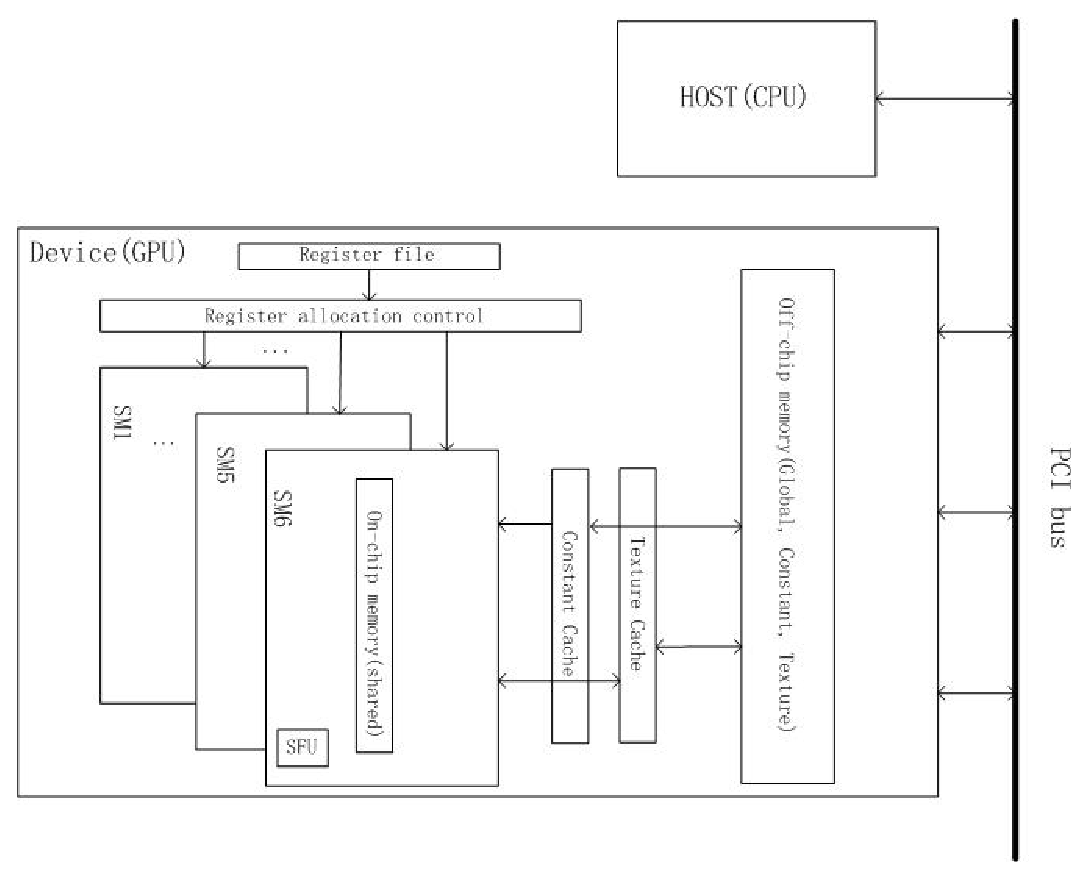
\includegraphics[scale=0.5]{High_view_of_CUDA_GPU_microarchitecture.eps}
\caption{High View of CUDA CPU Microarchitecture}
\label{figure2}
\end{figure}   
% Note that IEEE does not put floats in the very first column - or typically
% anywhere on the first page for that matter. Also, in-text middle ("here")
% positioning is not used. Most IEEE journals/conferences use top floats
% exclusively. Note that, LaTeX2e, unlike IEEE journals/conferences, places
% footnotes above bottom floats. This can be corrected via the \fnbelowfloat
% command of the stfloats package.
\section{GPU Based Acceleration of FCSD}
In this section we present the parallel implementation of fixed complexity sphere decoder by GPU, first from (\ref{formula 1}), the maximum likelihood (ML) solution is given by:
\begin{equation}
s_{ML}=arg\min_{s\in \mathbb{O}^{N_{t}}}||y-\mathbf{H}s||^{2} \label{formula 2}
\end{equation}
we consider the array $N_{t}=N_{r}$, performing QR decomposition to channel propagation matrix
\begin{equation}
 \mathbf{H}=\mathbf{Q}\mathbf{R}  \label{QR}
\end{equation}
where $\mathbf{Q}\in \mathbf{C}^{N_{t}\times N_{t}}$ is the unitary matrix, $\mathbf{R}\in \mathbf{C}^{N_{t}\times N_{t}}$, is the upper triangular matrix, the basing on \cite{matrix theory}, the (\ref{formula 2}) can be changed to
\begin{eqnarray}
\nonumber
s_{ML}&=&arg\min_{s\in \mathbb{O}^{N_{t}}}||\mathbf{Q}^{H}y-\mathbf{Q}^{H}\mathbf{H}s||^{2}\\
&=& arg\min_{s\in \mathbb{O}^{N_{t}}}||\mathbf{Q}^{H}y-\mathbf{R}s||^{2} \label{formula 3}
\end{eqnarray}
Consider the unconstrained estimation of $s$, $\hat{s}=\mathbf{G}y$, $\mathbf{G}=(\mathbf{H}^{H}\mathbf{H})^{-1}\mathbf{H}^{H}$ denotes the zero forcing equalizer, basing on \ref{QR}, we have  
\begin{equation}
\hat{s}=\mathbf{G}y=(\mathbf{R}^{H}\mathbf{R})^{-1}\mathbf{R}^{H}\mathbf{Q}^{H}y=\mathbf{R}^{-1}\mathbf{Q}^{H}y 
\label{unconstrained estimation}
\end{equation} 
Therefore $\mathbf{Q}^{H}y=\mathbf{R}\hat{s}$, the \ref{formula 3} can be changed to
\begin{equation}
s_{ML}=arg\min_{s\in \mathbb{O}^{N_{t}}}||\mathbf{R}(\hat{s}-s)||^{2} \label{formula 4}
\end{equation}
the Fixed Complexity Sphere Decoder works as a constant number of multiple path tree searching.
\begin{figure}[tb]
\centering
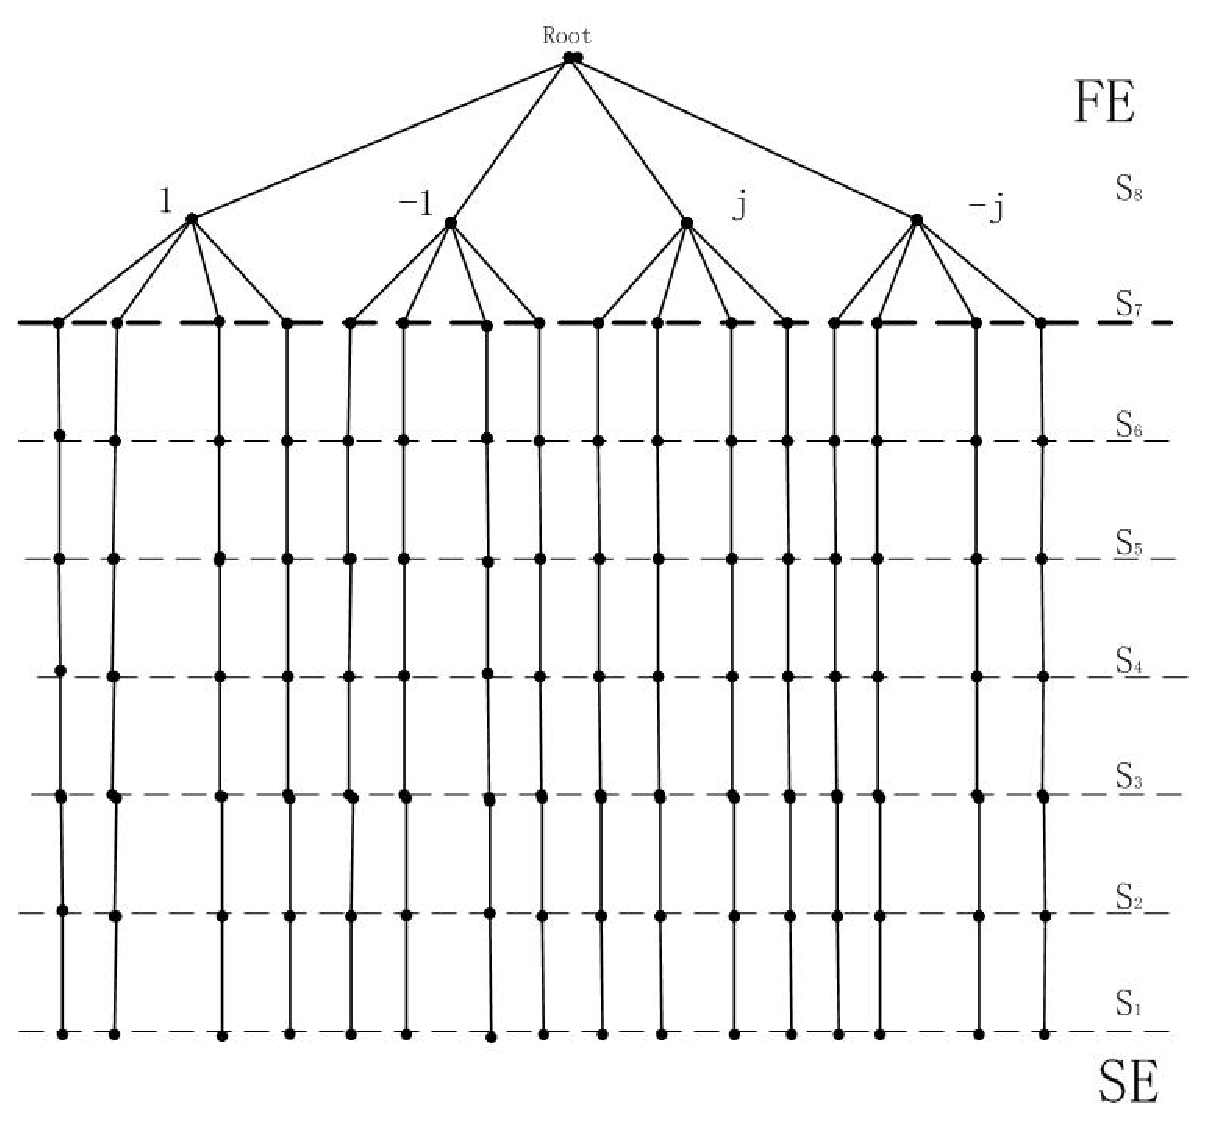
\includegraphics[scale=0.5]{FCSD_tree_searching.eps}
\caption{Tree searching of QPSK FCSD for 8x8 MIMO system}
\label{figure4}
\end{figure}
As shown in Figure \ref{figure4}, just like SD the FCSD also performs depth first searching, at the first $\rho$ level the FCSD search all the possible signal symbols $\widetilde{s}_{N_{t}} \widetilde{s}_{N_{t}-1}\dots \widetilde{s}_{N_{t}-\rho+1}$ in constellation $\mathbb{O}^{N_{t}}$, which is called Full Expansion(FE) level, the remain $N_{t}-\rho$ levels of symbols, the FCSD performs decision feed back equalization (DFE), from (\ref{formula 4}) the solution of FCSD can be given:
\begin{equation}
\hat{s}_{FCSD}=arg\min_{s\in \mathbb{O}^{N_{t}}}\sum_{i=1}^{N_{t}}|r_{ii}(\hat{s}_{i}-s_{i})+\sum_{j=i+1}^{N_{t}}r_{ij}(\hat{s}_{j}-s_{j})|^{2}  \label{formula 5}
\end{equation} 
$i\in [1,2\dots N_{t}]$, $r_{ij}$ denotes the element at the $i$th row and $j$th column of the upper triangular matrix $\mathbf{R}$, this process is called Single Expansion (FE).
thus the FCSD solution $s_{FCSD}=[s_{1},s_{2}\dots s_{N_{t}}]$ can be expressed as:
\begin{displaymath}
s_{FCSD}^{i}=\left\lbrace\begin{array}{c}
\in \mathbb{O}^{\rho}      \quad i=N_{t},N_{t}-1,\dots N_{t}-\rho+1\\
\mathbb{Q}[\hat{s}_{i}+\sum_{j=i+1}^{N_{t}}\frac{r_{ij}}{r_{ii}}(\hat{s_{j}}-s_{FCSD}^{i})] \quad i=N_{t}-\rho,N_{t}-\rho-1,\dots 2,1 \\
\end{array}\right.
\end{displaymath}
$\mathbb{Q}[]$ denotes the signal constellation based quantization. At the post processing stage, FCSD takes the symbol vector candidate with the minimum Euclidean metric $E_{metric}$:
\begin{equation}
E_{metric}=||\mathbf{R}(\hat{s}-\widetilde{s})||^{2}
\end{equation} 
The $\widetilde{s}$ denotes the symbol vector candidate, the total number of candidates is: 
\begin{equation}
M^{\rho}     \label{path number}
\end{equation} 
\subsection{CUDA-FCSD Pre-Prossing}
As shown in figure.4, each path of the FCSD searching has a serial execution nature, in order to avoid error propagation of decoder, FCSD ordering was applied to the propagation channel based on post processing signal to noise ratio\cite{Vblas}, which can be expressed as:
\begin{equation}
\varphi_{m}=\frac{E_{s}}{\sigma^{2}(\mathbf{H}^{H}\mathbf{H})_{mm}^{-1}}  \label{ppsnr}
\end{equation}
$\varphi_{m}$ denotes the post processing signal to noise ratio of the $m$th data stream, $(\mathbf{H}^{H}\mathbf{H})_{mm}^{-1}$ denotes the diagonal elements of the inversion of $HHH$ matrix $\mathbf{H}^{H}\mathbf{H}$, thus when the SNR is determined, the post processing SNR is only determined by $(\mathbf{H}^{H}\mathbf{H})_{mm}^{-1}$, for the FE stage the robustness of detector performance is not influenced by the post processing SNR thus at FE stage the "weakest" data stream is detected first, that is, the data stream with the smaller $\varphi$ is detected earlier. At SE stage, because of the single searching path of the symbol, the performance is tightly related to the post processing SNR, therefore at SE stage the data streams with the larger post processing SNR is detected earlier in order to avoiding the error propagation, in conclusion the FCSD ordering works iteratively  and obeys the following rule:
At the $j$th step ($j=1,2\dots N_{t}-1$), $s_{p}$ denotes the symbol to be detected, where 
\begin{displaymath}
p=\left\lbrace \begin{array}{c}
arg \max_{k}(\mathbf{H}_{j}^{H}\mathbf{H}_{j})_{kk}^{-1}\quad FE stage\\
arg \min_{k}(\mathbf{H}_{j}^{H}\mathbf{H}_{j})_{kk}^{-1}\quad SE stage \\  \label{the ordering}
\end{array}\right.  
\end{displaymath}  
$\mathbf{H}_{j}\in \mathbb{C}^{N_{r}\times (N_{t}-j+1)}$ denotes the renewed channel matrix, at the $j$th iteration with the column corresponding to previous detected data streams removed from $\mathbf{H}_{j-1}$.
the unconstrained estimation $\hat{s}$ in \ref{unconstrained estimation}  in is given by:
\begin{equation}
 \hat{s}=(\mathbf{H}^{H}\mathbf{H})^{-1}\mathbf{H}^{H}y \label{shat}
\end{equation}

Although the FCSD pre-processing has a serial nature and can not be vectorized, the computational consumptive operations \ref{the ordering} \ref{shat} can be implement by the CUDA Basic Linear Algebra Subprograms(cuBLAS), the matrix inverse(Gaussian Jordan Elimination) and cholesky factorization(Row Major Factorization) are also implemented by GPU, as shown in Table \ref{table 1}.
\begin{table}[htb]
\caption{Parallel Computation Operation of FCSD Pre-processing}
\centering
\begin{tabular}{|c|p{3cm}|p{3cm}|p{3cm}|p{3cm}|}
\hline
Operations & complex matrix-matrix multiplication & complex matrix-vector multiplication & matrix inverse & cholesky factorization \\
\hline
GPU subroutine & $\mathit{cublasCgemm}$  & $\mathit{cublasCgemv}$ & $\mathit{GJE}$ & $\mathit{chol}$\\
\hline
Formula   &  $\mathbf{H}^{H}\mathbf{H}$ & $(\mathbf{H}^{H}\mathbf{H})^{-1}\mathbf{H}^{H}y$ & $\mathbf{H}_{j}^{H}\mathbf{H}_{j})^{-1} $ & $\mathbf{H}^{H}\mathbf{H}=\mathbf{R}^{H}\mathbf{R}$ 
\\
\hline
  \label{table 1}
\end{tabular}
\end{table}

Figure \ref{block diagram} shows the block diagram of the CUDA-FCSD implementation, as mention in section \ref{programming model}, our implementation is based on heterogeneous programming principle, the flow control and logical operations are reside at the host side, the compute intensive works is implemented at device side.
\begin{figure}[htb]
\centering
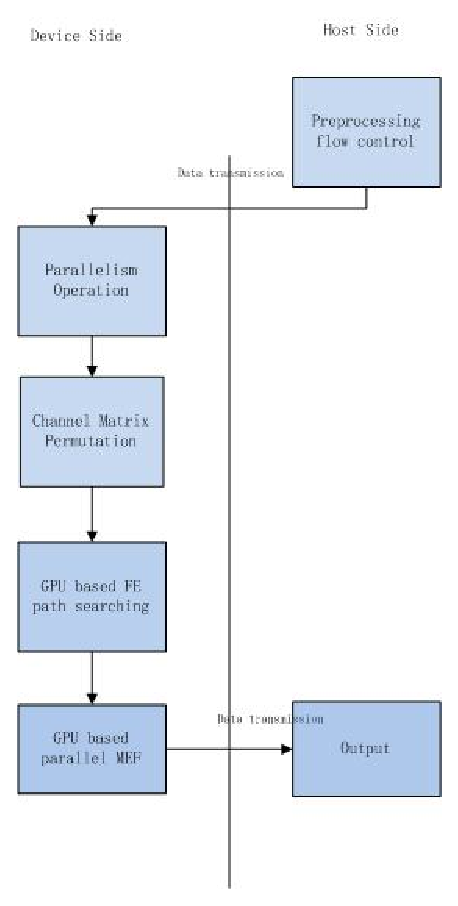
\includegraphics[scale=0.8]{CUDA_FCSD_block_diagram.eps}
\caption{Block Diagram of CUDA-FCSD Implementation}
\label{block diagram}
\end{figure}
\subsection{Parallel Acceleration of Blocked-Paths Searching}
  We consider $16\times 16$ MIMO system, the modulation scheme is $16$QAM, the path we need to search is $\mathbb{O}[M^{\rho}]=16^{3}=4096$, $\rho=\lceil \sqrt[2]{N_{t}}-1\rceil$, as mentioned in section \ref{programming model} the maximum number of threads that can be used in GPU is limited by the number of SM and maximum number of threads per SM, as to GeForce GTX 760. we have $12288$ threads totally.   For each path, decision feedback path searching has a serial nature, therefore we match path to one thread, in order to have largest amount of threads that can be paralleled, we use one dimension blocks for widest expansion and blocked all the paths into several one dimension blocks, for largest SM occupation we define 4 blocks for path searching kernel and each block has 1024 threads. At each path, we perform the following data operation:\\
1. \emph{Decision Feedback Equalization}\\
\begin{eqnarray}
\nonumber
{s}_{i}^{k}\in \mathbb{O}^{\rho}      \quad if\quad i&=&N_{t},N_{t}-1,\dots N_{t}-\rho+1\quad FE\\
\nonumber
{s}_{i}^{k}=\hat{s}_{i}^{k}+\sum_{j=i+1}^{N_{t}}\frac{r_{ij}}{r_{ii}}(\hat{s_{j}^{k}}-s_{j}^{k})\quad if\quad i &=& N_{t}-\rho,N_{t}-\rho-1,\dots 2,1\quad SE\\  \label{path searching}
\end{eqnarray}
$s_{j}^{k}$ denotes the $j$th symbol of the $k$th symbol vector candidate.\\
2. \emph{Euclidean Metric Calculation}\\
\begin{equation}
E_{u}^{k}=\sum_{i=1}^{i=N_{t}}\sum_{j=i}^{j=N_{t}}r_{ij}(\hat{s_{j}}-s_{j})\label{Eu metric}
\end{equation}
$E_{u}^{k}$ denotes the $k$th Euclidean metric of the corresponding symbol vector candidate $\widetilde{s}^{k}$. Then we take the symbol vector $s^{\theta}$ as the solution, where 
\begin{equation}
\theta=arg\min_{m}(E_{u}^{m})\quad m=1,2\dots M^{\rho} \label{Eu candidate}
\end{equation} 

\subsubsection{Data Preparation}
There are three major factors that will influence the configuration of the data set configuration in memory space.\\
1. Amount of Reading$\&$Writing operation per thread.\\
2. Program scope of the data.\\
3. Storage Requirement of data.\\
The memory reading$\&$writing (R/W) strategy of GPU is the crutial factor that influence the application performance because the GPU is data processing intensive and only has small cache for special memory space(constant, texture), another consideration is the validation life circle of data, local memory which is invoked in kernel function is valid in one thread, share memory is valid in one block, constant, texture and global memory are valid both at host side and device side. On the other hand different from global memory (2047 MBytes in GeForce GTX 760), the constant and share memory are all capacity limited (only $65536$ bytes totally and $49152$ bytes per block in GeForce GTX 760), so that for our application the configuration of memory is determined by the capacity requirement of the data. Here in table \ref{amount of R/W operation} we present the amount of R/W operations and the storage that needed for critical data variables in FCSD path searching. The amount of the R/W operation is calculated based on the (\ref{path searching}) and ((ref{Eu metric}), for complex value ($\mathbf{R}$,$\hat{s}$, $\mathit{s_{pontential matrix}}$,$\mathit{s_{kernel}}$ ) is stored use $\mathit{float2}$ which counts 8 bytes, floating point data set $E_{u}$ is stored in $\mathit{float}$, which counts for 4 bytes, $\mathit{s_{index}}$ is the integer list which is stored use $\mathit{int}$, which counts 1 byte. \\
 At host side we set 4 vector data set that are stored linearly in global memory which has program scope for both host side and device side, $\mathit{s_{potential matrix}}$ is used to store the $M^{\rho}\times N_{t}$ complex matrix that each row stores one symbol vector candidate and whose valid scope is through the whole kernel function. $\mathit{s_{index}}$, which is used to store the index of all the possible sub symbol vectors for  FE stage using full factorial method, requires a $\rho\times M^{\rho}$  integer matrix space.  $\mathit{E_{u}}$ is a $M^{\rho}$ floating point vector that is used to store the Euclidean metric of all the symbol vector candidates, obviously the valid scope of it is for the whole kernel function. $\mathit{s_{kernel}}$ is a complex vector used to store the FCSD solution which length is $N_{t}$ and has to be transferred to host side, thus it is also needed to be stored in global memory. \\
  On the other hand,   upper triangular matrix $\mathbf{R}$ in (\ref{formula 4})  and unconstrained estimation $\hat{s}$ in (\ref{unconstrained estimation})  requires a large amount of R operations and are read only. (for the $16\times 16$ $16QAM$ MIMO system the R/W of $\mathbf{R}$  and $\hat{s}$ are about  $370$ and $266$ per thread), these two data set need small size of storage(for the $16\times 16$ $16QAM$ MIMO system $1088$ bytes for $\mathbf{R}$ and $128$ bytes for $\hat{s}$  ) we make use of the read only constant memory to store the data which are capacity limited and do not need write operation in path searching , as we mentioned in section (\ref{programming model}), the constant memory is cached so that it is much faster than global memory.
 \begin{table}[htb]  
 \caption{Amount of R/W Operations and Storage Requirement of Different Data Set}
 \centering
\begin{tabular}{|p{3cm}|p{3cm}|l|p{3cm}|l|l|l|}
\hline
data & $\mathbf{R}$ & $\hat{s}$ & $\mathit{s_{pontential matrix}}$ & $\mathit{s_{index}}$ & $\mathit{E_{u}}$ & $\mathit{s_{kernel}}$ \\
\hline
R/W operations/thread & $(\frac{3}{2}(N_{t})^{2}-\frac{N_{t}}{2}+\rho-\rho^{2})$ & $(\frac{2(N_{t})^{2}+2N_{t}-\rho^{2}-\rho}{2})$ & $\rho$ & $N_{t}$ &$N_{t} $ & $N_{t}$ \\
\hline
Storage/bytes  & $4(N_{t}+1)N_{t}$ & $8N_{t}$ & $8M^{\rho}N_{t}$ & $N_{t}M^{\rho}$ & $4N_{t}M^{\rho}$ & $8N_{t}$\\
\hline  \label{amount of R/W operation} 
\end{tabular} 
\end{table} 
\subsubsection{Memory Accesss Pattern}
  When considering large MIMO array, the large amount of R/W operations determine that the memory bandwidth is the major bottleneck of the performance,  although the theoretical bandwidth of off-chip memory is extremely high (in GeForce GTX 760 the bandwidth of off-chip memory is around $192 GB/s$), however the effect memory bandwidth can only be achieved by proper R/W strategy.\\
  Global memory is implemented by dynamic random access memory (DRAM) whose R/W is extremely slow process, modern DRAM R/W data by access a pitch of consecutive memory location, as mentioned in section (\ref{programming model}), the warp is the basic schedule unit of device, with one instruction recall one warp of threads that execute at the same time, the most favorable global memory access pattern is to keep one warp of threads that access consecutive memory as much as possible, for GeForce GTX 760, the DRAM will access a consecutive memory address that has 128 bytes length, In Figure \ref{coalesce global memory} we take the global access pattern of the $\mathit{s_{potential matrix}}$ as an example to illustrate how we coalesce the the global memory,
we store $\mathit{s_{potential matrix}}$ in one pitch of linear global memory, with each row store one $N_{t}=16$ complex symbol vector solution candidate of $\hat{s}_{FCSD}$ in (\ref{formula 5}), totally there are $M^{\rho}=4096$ rows, this matrix is stored in column major. As mentioned before we operate one path in one thread, thus the address two consecutive symbol operated in one thread is $4096$, however for consecutive threads the address they reach is continues as shown in Figure \ref{coalesce global memory}, each 32 threads in one warp can make R/W operation to a pitch of continues memory, which is $32\times 8=256 bytes$, counts for two times of DRAM access.
\begin{figure}[htb]
\centering
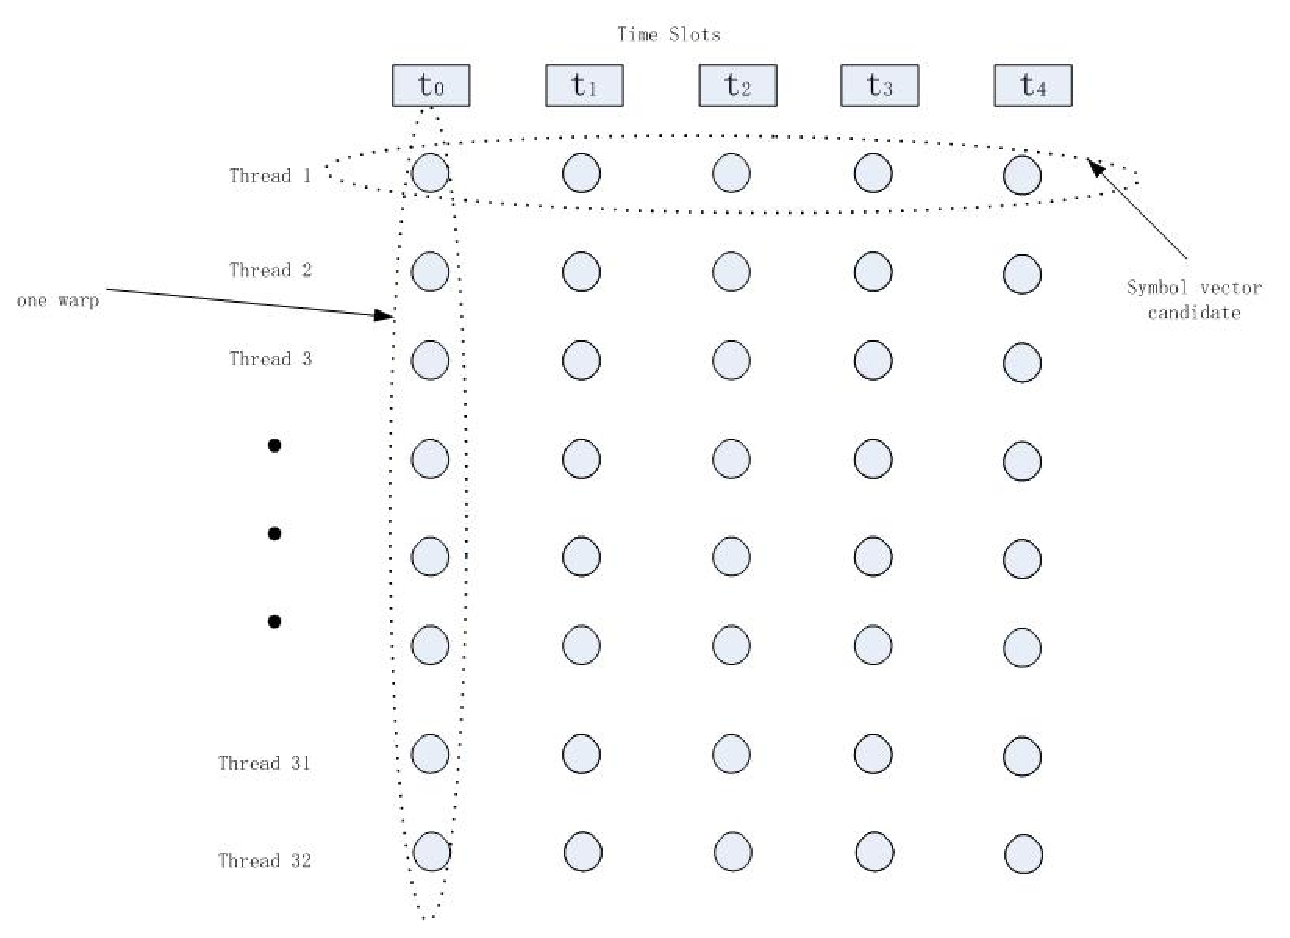
\includegraphics[scale=0.63]{coalescing_global_memory.eps}
\caption{Global Memory Access Pattern of $\mathit{s_{potential matrix}}$}
\label{coalesce global memory}
\end{figure}
 Another available resource for memory bandwidth increase is to make use of share memory, for all the transient variables that used for accumulator in (\ref{path searching}) and (\ref{Eu metric}), because of the small capacity consumption and large amount of R/W operations.   
\subsubsection{Data Transfer Minimization}   
The data transfer between the host side and the device side is much more slower than the inner device data transferring, therefore, in our application we minimize the data transferring times, we make data transfer only once for propagation channel matrix $\mathbf{H}$, received symbol vector $y$ in (\ref{formula 1}) as well as the index list $\mathit{s_{index}}$ at FE stage, we integrate the post processing (\ref{Eu metric}) into path searching kernel function to avoid the transferring of $E_{u}$ in (\ref{Eu metric}).  
\subsection{Going to Larger MIMO System}
  Consider the uplink $32\times 32$ MIMO system with $16$QAM modulation scheme, from \ref{path number}, the path number that need to be searched is $16^{5}=1048576$, as mentioned in section (\ref{programming model}), the maximum number of threads that can be execute in kernel function of GeForce GTX 760 is 12288, therefore we need to consider serial the one kernel into a certain times of loop, in order to avoid device synchronization latency, we synchronize and return the control to host side in order to reduce the synchronization expense. Under this condition we use 12 linear blocks and each block has 1024 threads, we execute the kernel function for 86 times and get the final solution.
\section{Simulation Results}
\subsection{Environment}
\subsubsection{Device}
\emph{Graphic Processing Units}: GeForce GTX 760, GPU clock rate: 1.08 GHz , memory clock rate: 3 GHz , number of SM: 6, maximum number of threads per stream multiprocessor: 2048, total amount of global memory: 2 GB, total amount of share memory per block: 49 KB, total amount of constant memory: 66 KB. \\
\emph{Central Processing Units-Modigliani}: Intel Core i5-4th generation, 4 cores 3.20 GHz CPU clock rate, 8 GB RAM\\
\emph{Central Processing Units-Monet} : Intel Core i7-3rd generation, 12 cores 3.20 GHz CPU clock rate, 32 GB RAM\\
\subsection{Software}
CUDA Driver Version / Runtime Version      6.5 / 6.0\\
Nsight Eclipse Version 6.5
\subsection{Performance and Evaluation}
\begin{table}[htb]
\caption{Speedup Performance of different MIMO Array size}
\centering
\begin{tabular}{|c|c|c|c|c|c|}
\hline
\multirow{2}{*}{ Array size} & \multicolumn{3}{|c|}{Time/s} & \multicolumn{2}{|c|}{Speedup}\\
\cline{2-6}
&GTX 760 & modigliani & monet & GTX/modigliani  & GTX/monet \\
\hline
$8\time 8$& 0.46& 0.09&0.08 & 0.20& 0.17\\
\hline
$16\time 16$&1.56 &3.2&3.57& 2.05& 2.29\\
\hline
$20\time 20$&31 & 74& 81& 2.39& 2.61\\
\hline
$25\time 25$& 38& 112& 122& 2.94& 3.21\\
\hline
$32\time 32$& 611&2836&3033&4.64& 4.96 \\
\hline
\label{speedup}
\end{tabular}
\end{table}
  \quad We test 5 array sizes and make comparison between GTX 760 and two kinds of CPU, all the operation times we test is based on 100 channel realizations, the transmitted data is generated randomly and modulated by $16$ QAM modulation scheme,  as we can see in \ref{speedup}, for small size array, like $8\times 8$, GPU has no advantage over CPU, for small array size, the number of path that need to be searched is relatively small, the CPU has already had a good performance, there is a short time for GPU to "warm up", for data transferring, launch kernel function and host device synchronization, further more, for small number of threads, the memory R/W latency is not well hided. When the array size grows large, a large parallelism is achieved so that the GPU begin to display its data processing power, and with the array size increasing, this speedup tends to be much more considerable.
\section{Conclusion}
In this paper, we present the GPU implementation of fixed complexity sphere decoder for a large MIMO system, which is a time consuming task for traditional platform, we have reached up to nearly 5 times acceleration of FCSD and this speedup grows higher with the increasing array size. In addition, the GPU and CPU can work independently, the data processing power of GPU computing is an extra bonus of the traditional simulation platform. This shows the potential of GPU computing for the simulation and consumptive computational work of large MIMO area.      
% conference papers do not normally have an appendix


% use section* for acknowledgement
%\section*{Acknowledgment}








% trigger a \newpage just before the given reference
% number - used to balance the columns on the last page
% adjust value as needed - may need to be readjusted if
% the document is modified later
%\IEEEtriggeratref{8}
% The "triggered" command can be changed if desired:
%\IEEEtriggercmd{\enlargethispage{-5in}}

% references section

% can use a bibliography generated by BibTeX as a .bbl file
% BibTeX documentation can be easily obtained at:
% http://www.ctan.org/tex-archive/biblio/bibtex/contrib/doc/
% The IEEEtran BibTeX style support page is at:
% http://www.michaelshell.org/tex/ieeetran/bibtex/
%\bibliographystyle{IEEEtran}
% argument is your BibTeX string definitions and bibliography database(s)
%\bibliography{IEEEabrv,../bib/paper}
%
% <OR> manually copy in the resultant .bbl file
% set second argument of \begin to the number of references
% (used to reserve space for the reference number labels box)






% that's all folks
\end{spacing}
\bibliographystyle{IEEEtran}
\bibliography{citation}
\end{document}


